%% You can use this file to create your answer for Exercise 1.  
%% Fill in the places labeled by comments.
%% Generate a PDF document by with the command `pdflatex ex1'.

\documentclass[11pt]{article}


\usepackage{times}
\usepackage{listings}
\usepackage{enumerate}
\usepackage{courier}
\usepackage{hyperref}
\usepackage{xcolor}
\usepackage{graphicx}


%% Values that are specific to a particular term
\newcommand{\thisterm}{Spring 2021}

\newcommand{\dateassigned}{Thur.,~Mar.~4}

%% Printed form of home page that students should use
\newcommand{\visiblecoursehome}{http://www.cs.cmu.edu/\textasciitilde{}418}

%% Link to home page that will stay valid
\newcommand{\actualcoursehome}{http://www.cs.cmu.edu/afs/cs.cmu.edu/academic/class/15418-s21/www}

\newcommand{\datedue}{Mon.,~Mar.~15}





%% Page layout
\oddsidemargin 0pt
\evensidemargin 0pt
\textheight 600pt
\textwidth 469pt
\setlength{\parindent}{0em}
\setlength{\parskip}{1ex}

%% Colored hyperlink 
\newcommand{\cref}[2]{\href{#1}{\color{blue}#2}}

%% Customization to listing
\lstset{basicstyle=\ttfamily\small,language=C,morekeywords={cilk_synch,cilk_spawn}}

%% Enumerate environment with alphabetic labels
\newenvironment{choice}{\begin{enumerate}[A.]}{\end{enumerate}}
%% Environment for supplying answers to problem
\newenvironment{answer}{\begin{minipage}[c][1.5in]{\textwidth}}{\end{minipage}}


\begin{document}
                          
\vspace*{0.3in}                            
\begin{center}
\LARGE
15-418/618 \thisterm{} \\
Exercise 4
\end{center}

\begin{center}
\Large        
\begin{tabular}{ll}
\hline             
Assigned: & \dateassigned{}  \\
Due: &  \datedue{}, 11:00~pm  \\
\hline       
\end{tabular}
\end{center} 

\section*{Overview}

This exercise is designed to help you better understand the lecture
material and be prepared for the style of questions you will get on
the exams.  The questions are designed to have simple answers.  Any
explanation you provide can be brief---at most 3 sentences.  You
should work on this on your own, since that's how things will be when
you take an exam.

You will submit an electronic version of this assignment to Canvas 
as a PDF file.  For those of you familiar with the \LaTeX{} text 
formatter, you can download the template and configuation files at: 
\begin{center} 
  \cref{\actualcoursehome/exercises/ex4.zip}{\visiblecoursehome/exercises/ex4.zip} 
\end{center} 
Instructions for how to use this template are included as comments in 
the file.  Otherwise, you can use this PDF document as your starting 
point.  You can either: 1) electronically modify the PDF, or 2) print 
it out, write your answers by hand, and scan it.  In any case, we 
expect your solution to follow the formatting of this document. 

\newpage 
\section*{Problem 1: Resource Oriented Scaling}
John Gustafson proposed a new formulation of speedup, in response to concerns about applying Amdahl's Law to some problem domains. For Gustafson's law, let $s$ be the fraction of execution that is inherently sequential (with dependencies preventing parallel execution), and $p$ be the speedup of the execution part that can benefit from from the improvement of computing resources. Then the speedup can be expressed as $S = s + (1-s)p$.

Compare briefly how the two scaling laws (Gustafson's and Amdahl's) relate to the scaling constraints taught in the lecture on workload-driven performance evaluation (\textbf{problem-constrained scaling, memory-constrained scaling and time-constrained scaling}).  Which constraint(s) is similar to the
scaling expressed by each law?  Why?
\begin{center}
\cref{\actualcoursehome/lectures/10_perfeval.pdf}{\visiblecoursehome/lectures/10\_perfeval.pdf}.
\end{center}

(Recall Amdahl's law: let s be the fraction of execution that is inherently sequential , then the maximum speedup in latency due to parallel execution is $S \leq 1/s$. More specifically, the speedup is $S \leq \frac{1}{s + \frac{(1-s)}{n}}$ where $n$ is the number of processors used.)

\begin{answer}
\begin{itemize} % amdahl's law
\item Problem Constrained Scaling: 
\begin{itemize}
\item Both Gustafson's and Amdahl's Law is similar to Problem Constrained Scaling because the speedup is proportional to number of processors.
\item Difference between two is that Gustafson's Law is more general than Amdahl's Law because it accounts for sequential part of the problem and
relative overheads, memory communication etc.
\end{itemize}
\end{itemize}

\end{answer}
\newpage 

\section*{Problem 2: Cache coherency}
\begin{choice}
  \item Your friend suggests modifying the MSI coherence protocol so that PrRd / BusRd behavior on the
  I-to-S transition is changed to PrRd / BusRdX, as is shown below:

\begin{center}
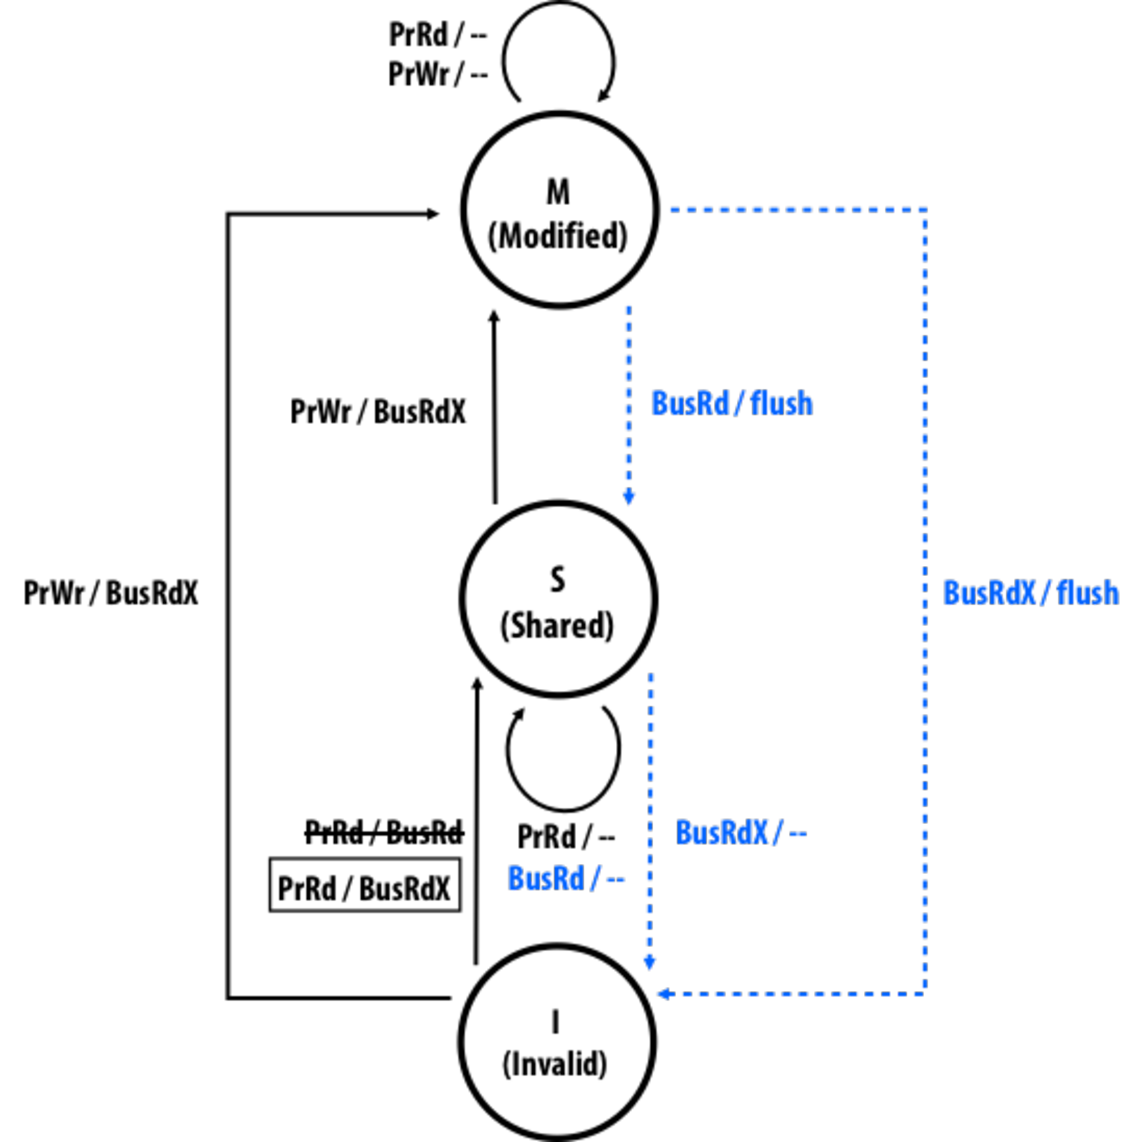
\includegraphics[width=3in]{msi.pdf} %% QUES
\end{center}





  Is the memory system still coherent? What impact does this change have on the system?

\begin{answer}
Memory system wouldn't be coherent because Shared state can modify the read values now. \newline
This implementation makes Modified state redundant.

\end{answer}

\item When we plot a parallel application’s cache miss rate as a function of the cache block size, we often see a U-shaped curve where the miss rate initially decreases with larger block sizes, but then it starts to increase. Please explain this phenomenon.

\begin{answer}
Since the cache block size increases, more values can be copied to cache at once. This decreases cache miss rate. \newline
But, if the cache block size is too large, then the cache will have to be flushed more often. This increases cache miss rate.\newline


\end{answer}


\end{choice}  


\end{document}
